\documentclass[sigconf]{acmart}
\usepackage{tikz}
\usepackage[ruled,vlined,spanish,onelanguage]{algorithm2e}
\usepackage{mathtools,nccmath}
\usetikzlibrary{arrows}

\AtBeginDocument{%
  \providecommand\BibTeX{{%
    \normalfont B\kern-0.5em{\scshape i\kern-0.25em b}\kern-0.8em\TeX}}}

\usepackage{graphicx}
\usepackage{background}
\backgroundsetup{contents=\includegraphics{logo.jpg}, scale=1, opacity=0.08, angle=0}
\begin{document}

%%
%% The "title" command has an optional parameter,
%% allowing the author to define a "short title" to be used in page headers.
\title{Artículo de Investigación: Clasificador de Texto}

\author{GIRÓN MÁRQUEZ, JOSÉ C.}
\email{jcgironma@correo.url.edu.gt}
\author{1064718}
\affiliation{%
  \institution{Universidad Rafael Landivar}
}

\author{VILLATORO MUÑOZ, ALEXANDER G.}
\email{agvillatoromu@correo.url.edu.gt}
\author{1182118}
\affiliation{%
  \institution{Universidad Rafael Landivar}
}

\author{DAMIAN CRUZ, KEVIN A.}
\email{kadamian@correo.url.edu.gt}
\author{1059116}
\affiliation{%
  \institution{Universidad Rafael Landivar}
}
\author{CORTEZ JUÁREZ, GÉNESIS D.}
\email{gdcortez@correo.url.edu.gt}
\author{1059618}
\affiliation{%
  \institution{Universidad Rafael Landivar}
}
\author{IZABEL PAIZ, KAREN I.}
\email{kipaiz@correo.url.edu.gt}
\author{1215718}
\affiliation{%
  \institution{Universidad Rafael Landivar}}

%%
%% The abstract is a short summary of the work to be presented in the
%% article.
\begin{abstract}
En el proyecto final del curso de Inteligencia Artificial de la Universidad Rafael Landivar, la cual tiene como objetivo implementar un agente inteligente y poder entrenarlo utilizando el Teorema de Bayes y Naive Bayes, esta práctica fue realizada a cargo de un grupo de estudiantes de la Sección 2.

Para poder realizar tal proyecto se investigó y estudió diferentes temas, en los cuales fueron el Teorema de Bayes en el cual no habla sobre poder calcular la probabilidades de un efecto teniendo información de antemano sobre las causas de este, otro tema investigado para la realización del proyecto y uno de los más importantes es “Naive Bayes” o clasificador de texto en el cual nos da a entender que es un clasificador probabilístico fundamentado en el teorema de Bayes, que suele asumir que las variables predictoras son independientes entre sí.

El proyecto se realizó en el lenguaje de programación Java en el cual consistió en que el sistema se tendrá que entrenar durante la prueba con archivos diferentes que se deben de cargar, por lo cual se ingresa un archivo con frases a clasificar con sus etiquetas respectivas, y sus frases, contando la cantidad de palabras que se repiten en esa etiqueta y la cantidad total de palabras que se ingresaron en esta, por este motivo se logró el cálculo de la probabilidad de cada palabra dada la etiqueta ingresada, posteriormente con las probabilidades calculadas de cada palabra lograr usar el algoritmos de Naive Bayes para poder clasificar dichas frases ingresadas más adelante.

Al realizar dicho entrenamiento del agente inteligente, se ingresará un texto o una frase en la cual nos identificará el tipo de texto que se está escribiendo o en este caso su etiqueta correspondiente. 

\end{abstract}
\maketitle
%%
%% Keywords. The author(s) should pick words that accurately describe
%% the work being presented. Separate the keywords with commas.
\section{KEYWORDS}
\textbf{Teorema de Bayes:} Es el caso en donde se desea calcular la probabilidad posterior de que ocurra un cierto evento A, dadas algunas probabilidades de eventos anteriores. 

FORMULA
\begin{equation}
\label{eq:bayes1}
P(A|B) = \frac{P(A)P(B|A)}{P(B)}
\end{equation}

\textbf{Probabilidades:} es la parte de las matemáticas que se encarga del estudio de los fenómenos o experimentos aleatorios. Por experimento aleatorio entenderemos todo aquel experimento que cuando se repite bajo las mismas condiciones iniciales, el resultado que se obtiene no siempre es el mismo. 

\textbf{Clasificador bayesiano ingenuo (Naive Bayes):} Naive Bayes es una técnica de clasificación y predicción probabilística de aprendizaje automático, o Machine Learning fundamentado en el teorema de Bayes. Utiliza datos históricos para construir modelos y encontrar asociaciones y relaciones para hacer predicciones.

\textbf{Machine Learning o aprendizaje supervisado:} Es una disciplina del campo de la Inteligencia Artificial que, a través de algoritmos, enseña a los agentes inteligentes la capacidad de identificar patrones en datos masivos para hacer predicciones. El aprendizaje o enseñanza consiste en la capacidad del sistema para identificar una gran serie de patrones complejos determinados por una gran cantidad de parámetros.\citep{Roman}


%%
%% This command processes the author and affiliation and title
%% information and builds the first part of the formatted document.

\section{Introducción}
En el proyecto final de Inteligencia Artificial se realizará una serie de procesos en donde se trabajará el tema de Naive Bayes y Probabilidades. Este proyecto final tiene como objetivo poder determinar el tipo de texto que se ingrese dependiendo del entrenamiento que se esté realizando.

El proyecto consistirá en diferentes procesos. En el primer proceso consistirá en ingresar un archivo de datos que contengan una frase y su etiqueta para poder entrenar al agente inteligente, como segundo punto con ayuda de esos datos ingresado, se estará calculando la probabilidad de cada palabra ingresada dada su etiqueta para poder saber la probabilidad para esto se necesita saber la cantidad de veces que la palabra aparece en la cantidad total de palabras que se ingresaron de esa etiqueta y con esto poder saber la probabilidad en el cual nos ayudará en el algoritmo de “Naive Bayes”, posteriormente se ingresa una frase sin etiqueta en la cual se estará comparando palabra por palabra para poder identificar de qué tipo de etiqueta corresponde gracias a las probabilidades calculadas por el archivo de entrenamiento.

El Naive Bayes trata sobre una técnica de clasificación de texto en la cual se puede predecir en base a un aprendizaje para el agente inteligente utilizando el teorema de Bayes. La traducción al español sobre “Naive Bayes” es “ingenuo” ya que nos da a entender que las variables son independientes entre sí.

En este proyecto se buscará mostrar la correcta clasificación de texto dependiente del entrenamiento dado al agente inteligente, y poder entender que con las probabilidades nos pueda dar una mejor decisión o camino para nuestro agente.\citep{Space}
\section{Estado del Arte}
\subsection{Clasificador Semi-Naive Bayes con Multiresolución para la Estimación de Estados Afectivos: Aplicación en Rehabilitación Virtual}
Jesús Joel Rivas para su maestría en ciencias de la computación del Instituto Nacional de Astrofísica, Óptica y Electrónica establece “Las emociones tienen influencia en la vida de los seres humanos, aún la voluntad para realizar actividades cotidianas se ve alterada por el estado de ánimo”. A base de esto comienza con la investigación del cómputo efectivo, área dedicada a identificar y simular estados emocionales de las personas por medio del uso con la computadora. Buscando la implementación de esta área en las terapias de recuperación de las personas ya que logra adaptarse a las necesidades del paciente.

En su investigación se estudia, mediante técnicas de aprendizaje de máquina, la relación de los movimientos de la mano y presión de los dedos del paciente, con los 4 estados afectivos escogidos: cansancio, ansiedad, dolor y motivaci´on; y se propone un modelo computacional binario (ausencia o presencia del estado afectivo) que alcance la mejor clasificación posible, para cada estado afectivo considerado.

Durante el proceso utilizó: Receiver Operating Characteristic Area Under the Curve, Naive Bayes con mejoramiento estructural y Semi-Naive Bayes. Dando un resultado a favor P1 de 0.897 ± 0.144 y para P2 de 0.691 ± 0.153 por Semi-Naive Bayes. Los resultados permiten sugerir que la motivación y el cansancio son susceptibles para la clasificación a partir del flujo de los datos observables de los movimientos y presión de la mano abriendo la posibilidad de decodificar el estado afectivo y explotar esa información para la adaptación de la terapia. Este conocimiento puede ayudar a mejorar el desarrollo de interfaces adaptables e inteligentes.\citep{Lee}\citep{Lopez}

\subsection{Clasificador Jerárquico de Imágenes utilizando Naive Bayes}
Según estudios de Julio Hernandez, junto a Maribel Marin, existen áreas en donde es
indispensable la manipulación de información para solucionar un
problema determinado, tal es el caso de la clasificación de imágenes.
Dicho proceso de clasificación una instancia puede ser clasificada en
más de una clase. La clasificación jerárquica proporciona una solución
a este problema ya que permite la combinación de información entre
clases que mantienen una relación jerarquica. Esto permite una mejor
clasificación de una instancia, evitando que esta sea ambigua. Los autores han propuesto como solución a este problema un enfoque basado en clasificadores encadenados. Este enfoque
permitió combinar la información de las clases. Para lograr esto
se desarrolló un modelo donde cada nodo, dentro de una jerarquía,
corresponde a un clasificador Naive Bayes, el cual compartía la
información resultante a sus nodos hijos.

Al finalizar el proyecto se obtuvieron resultados exitosos logrando que la clasificación mejorara considerablemente con respecto a una clasificación que solo involucrara la utilización del clasificador Naive Bayes. Una de las observaciones finales fue que utilizar un enfoque tanto de jerarquía como de encadenamiento en un proceso
de clasificación es un campo prometedor de buenos resultados. Sin embargo, en la fase de resultados se pudo notar que el número de objetos de una clase influía en la clasificación aún cuando el porcentaje de la misma fue elevado. L\citep{Noe}



\section{Modelos Culturales Propuestos}
\subsection{Un modelo basado en el Clasificador Naïve Bayes para la evaluación del desempeño docente}
La retroalimentación hacia los docentes por parte de los alumnos es un tema con bastante importancia en latinoamérica ya que brinda la oportunidad a los docentes a mejorar su desempeño y en ocasiones a sentirse halagados por los buenos comentarios que reciben de los alumnos. Este modelo describe el desarrollo y evaluación de un Modelo Computacional denominado SocialMining, basado en el algoritmo Naive Bayes, para apoyar el análisis de las opiniones de los estudiantes en el proceso de la evaluación del desempeño docente, llevada a cabo mediante dispositivos móviles. Dicho modelo se alimenta con evaluaciones pasadas las cuales permiten poder dar un mejor resultado aunque actualmente cuenta únicamente con los niveles: Positivo, Negativo y Neutral. Para medir el desempeño del proceso de clasificación del Modelo Computacional SocialMining, se utilizan métricas como la matriz de confusión, precisión y la curva de ROC. Los resultados obtenidos durante las pruebas del modelo arrojaron resultados positivos por los tester haciendo de este considerablemente factible para las instituciones de estudios superiores. 

La evaluación docente contribuye al fortalecimiento de las prácticas de enseñanza, además de que permite orientar la formación continua y sirve como un marco de referencia del desempeño del docente. Cabe resaltar que dicho modelo tuvo una alimentación innovadora ya que además de la recolección de puntaje hacia docentes y comentarios, lo alimentaron por medio de tweets de estudiantes hacia los catedráticos de sus años.

El Modelo Computacional SocialMining presenta ventajas frente al análisis de opiniones de estudiantes, debido a que comúnmente es realizado por personas, el apoyo con sistemas de información programados implica menor tiempo invertido y se tiene como resultado una evaluación cualitativa; esto permite implementar acciones correctivas y/o preventivas en la actividad docente en un tiempo más efectivo.\citep{Rincon}\citep{Lou}\citep{Gupte}


\section{Marco Teórico}
\subsection{Naive Bayes}
Naive Bayes es una técnica de clasificación y predicción probabilístico de aprendizaje automático, o Machine Learning fundamentado en el teorema de Bayes. Utiliza datos históricos para construir modelos y encontrar asociaciones y relaciones para hacer predicciones. Estos modelos Bayesianos son llamados algoritmos “Naive”, o “Inocentes”, debido  a que en ellos se asume que las variables son independientes entre sí. En otras palabras, que la presencia de una característica en un conjunto de datos no está en absoluto relacionada con la presencia de cualquier otra característica. En la implementación de un clasificador de texto, este no es el caso, ya que ciertas palabras en cada idioma suelen aparecer juntas con frecuencia, sin embargo, en la práctica funciona bastante bien y es la forma más fácil de construir modelos debido a su simplicidad.

Al aplicar el teorema de Bayes, se desea calcular la probabilidad ‘posterior’ de que ocurra un cierto evento A, dadas algunas probabilidades de eventos ‘anteriores’. En el caso del clasificador de texto, la probabilidad de que un mensaje pertenezca a una etiqueta. Por lo tanto, para cada palabra W en una etiqueta E, se realizaría el cálculo tal y como se muestra en la figura 1. \citep{Rincon}\citep{Roman}

Figura 1
\begin{equation}
\label{eq:bayes}
P(E|W) = \frac {P(W|E) P(E)} {P(W)}
\end{equation}

Considerando a una frase, como un conjunto de palabras {W1, W2, … Wn} y considerando una etiqueta en concreto, nos interesa obtener

FÓRMULA LATEX 
\begin{equation}
\label{eq:bayes1}
P(E|W_1, W_2, ... W_n)
\end{equation}
Para la cual, se debe crear la red bayesiana expresada en la figura 2.
\begin{center}
Figura 2
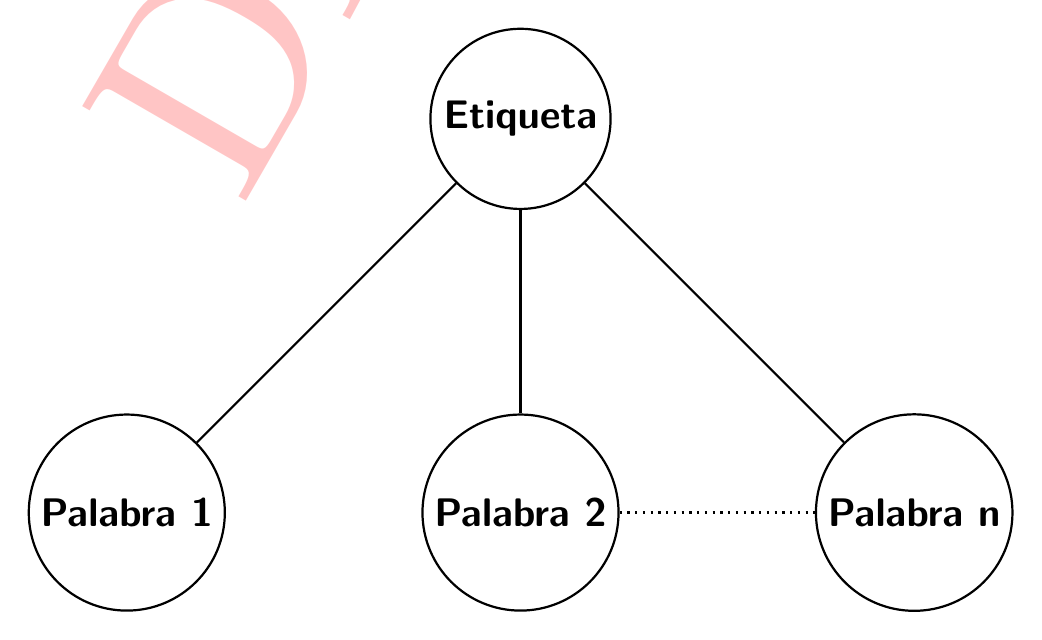
\begin{tikzpicture}
[-,>=stealth',auto,node distance=5cm,
                    thick,main node/.style={circle,draw,font=\sffamily\Large\bfseries}]

  \node[main node] (1) {Etiqueta};
  \node[main node] (3) [below of=1]{Palabra 2};
  \node[main node] (2) [left of=3] {Palabra 1};
  \node[main node] (4) [right of=3] {Palabra n};

  \path[every node/.style={font=\sffamily\small}]
    (1) edge node [right] {} (4)
        edge node [left] {} (2)
        edge node [below] {}(3)
    (3) edge [dotted] node[right] {} (4);
\end{tikzpicture}
\end{center}
Expresándose para un mensaje completo como se muestra en la figura 3.
\begin{center}
Figura 3
\begin{equation}
\label{eq:bayes2}
P(E|W_1, W_2, ... W_n) = 
\frac {P(W_1, W_2, ... W_n|E)P(E)} {P(W_1, W_2, ... W_n|E_1)P(E_1)+... +P(W_1, W_2, ... W_n|E_n)P(E_n)}
\end{equation}
\end{center}
De forma más general, la probabilidad para una etiqueta en específico se expresaría como se muestra en la figura 4.

Figura 4
\begin{equation}
\label{eq:bayes3}
P(E|W_1, W_2, ... W_n) = \frac {\prod_{i=1}^{n} P(W_i|E) P(E)} {\sum_{j=1}^{m} \prod_{i=1}^{n} P(W_i|E_j) P(E_j)}
\end{equation}

Considerando que el proceso se repite para cada etiqueta que se encuentra dentro del modelo y que posteriormente el resultado de cada probabilidad obtenida será comparado para seleccionar el que más se ajuste, se puede simplificar el cálculo al identificar un patrón.  En la práctica, si lo único que se desea es obtener la probabilidad mayor, se puede eliminar el denominador, éste se repite en cada uno de los cálculos, es decir, se mantiene constante. Por tanto, lo único que se está comparando es el numerador. De esta forma, el numerador sería equivalente a una probabilidad compuesta, y en su forma más general se expresaría como se muestra en la figura 5.\citep{Lee}\citep{Lopez}

Figura 5

\begin{equation}
\label{eq:bayes4}
{Mejor\;valor} = Max(P(E) \prod_{i=1}^{n} P(W_i|E))  
\end{equation}
\subsection{IMPLEMENTACIÓN}
Proceso de entrenamiento y clasificación de texto. El proceso de entrenamiento consiste en la carga de un archivo txt en formato csv el cual contiene frases en diferentes idiomas, debidamente identificadas. Se obtiene la probabilidad condicional de cada palabra y la probabilidad de cada etiqueta.Creando así el modelo. Para una frase no identificada se aplica la fórmula de Bayes presente en la figura 5 para cada etiqueta, esto representa un puntaje que se tomará como referencia para predecir el idioma del texto. Se tomará como resultado la frase con el mayor puntaje.\citep{Gupte}\citep{Space}
\newline
\newline
\newline
\newline
\newline
\newline
\newline
\newline
\newline
\newline
\newline
\newline
\newline
\newline
\newline
\newline
\newline
\newline
\newline
\newline
\begin{algorithm}[H]
\SetAlgoLined
 Inicio\;
 
 \ForEach{Etiqueta E en Entrenamiento}
 {
     \ForEach{Palabra W en Entrenamiento}
     {
            \begin{fleqn}[\dimexpr\leftmargini-\labelsep]
            \setlength\belowdisplayskip{0pt}
            \begin{equation}
                  Obtener: P(W|E) = \frac {|Frecuencia\;de\;W| + 1} {|Palabras\;en\;E| + |Cantidad\;Etiquetas|}
            \end{equation}
            \end{fleqn}%
     }
     
    \begin{equation}
            Obtener: P(E) = \frac {|Palabras\;en\;E|} {|Palabras\;Totales|}
    \end{equation}
 }
 \caption{Entrenamiento}
\end{algorithm}



\begin{algorithm}[H]
\SetAlgoLined
\KwResult{Predicción}
 \ForEach{Etiqueta E en Modelo}
 {
        Resultado = P(E)
    
     \ForEach{Palabra W en Texto}
     {
            Resultado *= P(W|E)
     }
     
    \eIf{es el mayor}
    {
        Predicción = E
   }
   {
   Descartar
   }
 }
 
 \caption{Clasificación de texto}
\end{algorithm}

\textbf{Corrección de muestras}

Antes de hacer cualquier análisis, es necesario hacer un ajuste a los datos recibidos y hacerlos estándar, es decir, hacer operaciones para que no distinga entre minúscula y mayúscula y eliminar caracteres especiales que no son propios del lenguaje, tales como signos de puntuación. Si el valor de la clase y de la función dada no ocurren juntas en los datos de entrenamiento, entonces la estimación basada en la probabilidad de frecuencia será cero. Esto representa un problema, ya que al multiplicarse con otros datos hará de toda la probabilidad cero, sin importar si otras palabras en el texto daban mejores resultados. Por lo tanto, se realiza una corrección al cálculo de probabilidad condicional de la palabra W en la etiqueta E de manera que este nunca dé como resultado cero, para ello, todo lo relacionado al conteo de frecuencias tiene como valor inicial 1. De esta manera, ninguno de los cálculos tendrá un numerador de 0. Esto sobreestima la probabilidad para dicha palabra, por lo que también se agrega al total de etiquetas disponibles al denominador. Se realiza este último paso porque implícitamente se está realizando un seguimiento de varias cosas: la cantidad de idiomas que contienen esa palabra y la cantidad que no. La suma de esas dos cosas debe estar en el denominador como se expresa en la figura 6.\citep{Apd}

Figura 6

\begin{equation}
\label{eq:bayes5}
P(W|E) = \frac {|Frecuencia\;de\;W| + 1} {|Palabras\;en\;E| + |Cantidad\;Etiquetas|}
\end{equation}

\textbf{Problema de underflow en punto flotante}

Multiplicar un set de probabilidades (figura 5) resulta ser un problema cuando se tienen muchos datos, ya que al tratarse de números tan pequeños, la estructura donde se almacenaría el resultado no lo soportaría y el resultado de la multiplicación terminaría siendo aproximado a 0. Para resolver este problema, se aprovechan las propiedades de los logaritmos, para obtener un puntaje proporcional que sí soportaría el programa. Para ello, se realiza la operación presente en la figura 7, en lugar de la descrita en la figura 5.
 \newline
 \newline
 \newline
 \newline
 \newline
\begin{equation}
\label{eq:bayes6}
{Mejor\;valor} = Max(log(P(E)) + \sum_{i=1}^{n} log(P(W_i|E)))  
\end{equation}

\textbf{Problemática}

La clasificación de texto es una de las principales aplicaciones de la inteligencia artificial. En donde basados en textos de entrada un agente inteligente puede realizar diferentes tareas de inferencia y recomendación, tales como la detección de idiomas.
El proceso para la detección o recomendación de idiomas es el siguiente:

Entrenamiento, mediante entradas de texto que representan tanto frases como etiquetas, entrenamos a nuestro agente inteligente.
Recomendación, en base a la normalización de los datos y la creación de un modelo bayesiano capaz de generar una recomendación según la entrada a evaluar.

Además, cabe recalcar que para obtener mejores recomendaciones, se necesita un entrenamiento más exhaustivo, en donde debemos ingresar una cantidad más elevada de muestras a nuestro agente inteligente.


\textbf{Propuesta de trabajo}

Justificación: 
Un motor de recomendación, mediante el ingreso de frases sin contexto y etiquetas, puede generar un modelo bayesiano capaz de inferir y con esto, según la entrada a evaluar que proporcione el usuario, generar una recomendación.

\textbf{Objetivo:}
Crear un sistema de recomendación que pueda ser entrenado y que utilice un agente inteligente para generar recomendaciones según la interacción con el usuario.

\textbf{Desarrollo:}
Los procesos en los que se desglosa el sistema son:
Lectura de archivo CSV
Organización de los datos
Cálculo de probabilidades de cada frase
Aplicacion de modelo Bayesiano
Lectura de palabra a evaluar
Respuesta con la recomendación final
 \citep{Gupte}

\section{Resultados esperados y obtenidos / Evaluación}

Con el algoritmo previamente descrito, se ha realizado la implementación del agente inteligente en el lenguaje de programación Java. Se realizó la implementación de una interfaz gráfica la cual contaba con una entrada para el archivo de entrenamiento en formato csv. Una vez elegido el archivo, este se carga al programa para su lectura y clasificación de palabras según la etiqueta proporcionada. Una vez se ha cargado al programa un archivo, se genera la probabilidad condicional de cada palabra para cada idioma en el cual tiene aparición.
Con la estructura de Bayes generada, el usuario a través de la interfaz implementada podrá ingresar frases para determinar la etiqueta que mejor se adecue. Con la frase ingresada, el programa recupera cada una de las palabras en esta y con la implementación de la figura 7 determina la probabilidad conjunta para cada uno de los idiomas en la estructura. El programa a través de la interfaz gráfica muestra al usuario el idioma con la mayor probabilidad obtenida. La interfaz también ofrece información adicional de los idiomas con adicionales y las probabilidades de que la frase pertenezca a estos.
Con esta implementación se obtuvo un agente inteligente que determina el idioma de una frase después de un entrenamiento previo. 


\section{Conclusiones}
\begin{itemize}
\item Los agentes inteligentes a través del teorema de Bayes son capaces de clasificar estructuras según una etiqueta y hacer inferencias probabilísticas.
\item Los agentes inteligentes necesitan una carga previa de datos para generar inferencias.
\item Los agentes inteligentes pueden ser herramientas de gran utilidad para optimización de procesos, análisis de información e inferencia de la misma.
\item Mientras más información se le proporcione al agente inteligente, este realizará mejores inferencias. 
\end{itemize}


\section{Trabajos Futuros / Recomendaciones}

Para futuros trabajos e implementaciones se recomienda a los lectores de este trabajo la aplicación de logaritmos para evitar problemas con los decimales que aproximen a 0. Esta implementación fue ilustrada en la sección de Problema de underflow en punto flotante del presente informe.
Se recomienda también la alimentación del agente inteligente con grandes volúmenes de datos. A mayor cantidad de información es proporcionada al agente por cada etiqueta, generará inferencias más acertadas. 
Los resultados están basados en los datos ingresados al sistema por lo que se recomienda que las pruebas realizadas estén basados en estos. Se recomienda también que se entrene varias veces una misma operación para generar mayor probabilidad anidada al idioma deseado en caso de la aparición de etiquetas erróneas.

\bibliographystyle{ACM-Reference-Format}
\bibliography{references}
\end{document}
\endinput

